\subsection{Ausblick  und erstes Konzept der praktischen Umsetzung}\label{technGrundkonzept}
Nachdem in den vorherigen Kapiteln einzelne Aspekte der Wertschöpfungskette erläutert wurden, soll es abschließend einen Ausblick auf die Bachelorarbeit geben und ein erstes technisches Konzept des Prototypen vorgestellt werden. Im Laufe der Arbeit haben sich einige zu erläuternde Aspekte aufgetan, welche aus Platzgründen erst in der Bachelorarbeit behandelt werden.\\

Im Rahmen dieser soll zunächst ein erster Zyklus des UCD durchgeführt werden, um so die Nutzeroberfläche der Mensch-Maschinen-Schnittstelle zu erarbeiten. Dabei sollen zusätzlich mögliche Personalisierungsfeature benannt werden. Weiterhin sollen die anderen im Folgenden vorgestellten Teilsysteme entwickelt werden. Unter anderem soll ein Suchalgorithmus für den SUPR des Servers erarbeitet werden sowie eine Gegenüberstellung von Rechenleistung und Sendeleistung des Autos bzw. des Servers erfolgen. Es werden die einzelnen Bausteine einer Wertschöpfungskette (zur Erkennung
und Bereitstellung neuer Fahrumfänge intelligenter Fahrzeug) benannt, erläutert und im Prototypen veranschaulicht. Im Folgenden wird für diesen ein erstes technisches Konzept vorgestellt.\\

\begin{large}
	\textbf{Erstes technisches Konzept des Prototypen}\\
\end{large}
Abbildung \ref{konzept} zeigt eine erste Architektur des Prototypen. Dieser ist unterteilt in das \textbf{Fahrzeug}(unten) und den \textbf{Server}(oben). Das Fahrzeug ist in drei Teilsysteme aufgeteilt. Der "Carla Python Skript Client" ist das Modul in dem die Simulation stattfindet. Entscheidungen bzgl. der Fahraufgabe werden in diesem getroffen. Die \textbf{Mensch-Maschine-Schnittstelle} ist eine Android-basierte App. Sie wird über einen Emulator bedienbar sein und soll unter anderem Informationen aus dem Carla Simulator darstellen. Damit dies möglich ist, wird der dritte Baustein des Fahrzeugs eingeführt: der SUPR.\\
Der SUPR des Fahrzeugs soll die im Forschungsseminar definierten Aufgaben durchführen können und dient zusätzlich als Kommunikationseinheit. Er verbindet die Carla Simulation und die Mensch-Maschine-Schnittstelle, sodass eine interne Kommunikation im Fahrzeug möglich ist. Desweiteren dient der SUPR als Kommunikationseinheit zum Server. Er ist für die Installation eingehender Softwarevorschläge zuständig und muss entsprechende Updates an den Python Client senden. In der Uptane Architektur waren hier die ECU's eines Autos angedacht. Da diese in dem ersten Konzept nicht auftauchen, steuert dies der SUPR.
\begin{figure}[H]
	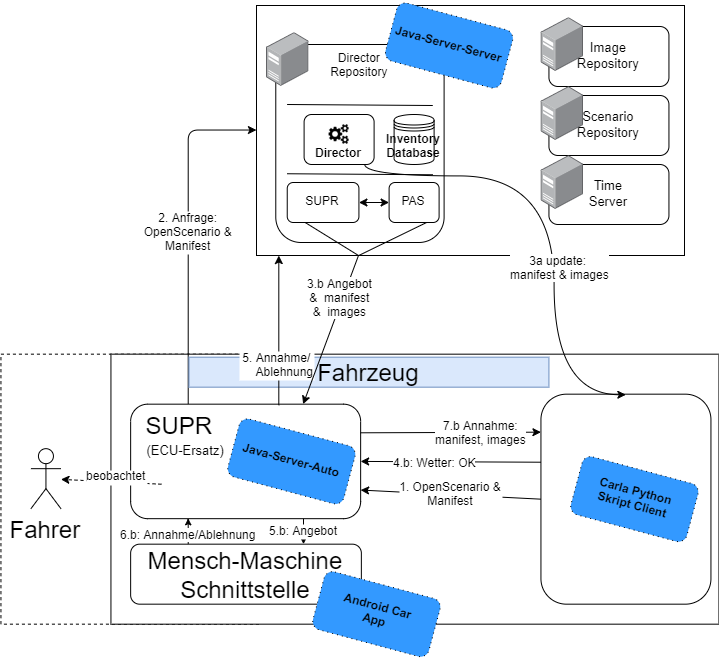
\includegraphics[width = \linewidth]{../pictures/konzept.png}
	\caption{Technisches Erstkonzept}
	\label{konzept}
\end{figure}
Die Architektur des Servers ist identisch zu der aus Kapitel 3.2. In der Implementierung sollen der Einfachheit halber die vier Bestandteile des Servers auf einem Server laufen und nicht getrennt werden. Der SUPR des Director Repositorys soll die im Forschungsseminar ihm zugeschriebenen Aufgaben durchführen können, gleiches gilt für den PAS. Die einzelnen Bestandteile des Servers können mit Ausnahme des Time-Servers miteinander kommunizieren.\\
Aus den Pfeilen des Konzepts abzuleiten ist der mögliche Ablauf eines Kaufprozesses. Initiiert wird dieser dadurch, dass das Fahrzeug im Carla Client nicht mehr autonom Fahren kann. Dieser erstellt infolgedessen eine OpenScenario-Datei und schickt diese gemeinsam mit dem Manifest, in welchem die bereits installierte Software notiert ist, an den SUPR (Pfeil 1). Dieser schickt den entdeckten Bedarf als Anfrage an den Server (Pfeil 2), welcher infolgedessen überprüft welche Software den entdeckten Bedarf abdecken kann. Hierzu sucht der Director des Servers im Manifest des Fahrzeugs nach zu aktualisierender Software. Wird ein Defizit festgestellt, stellt der Server eine Verbindung mit dem Python Client her, welcher dieses Update installiert (Pfeil 3.a). Ist jede Software wieder aktuell stellt der SUPR des Servers fest, ob die Bedarfssituation mit den Updates bewältigt werden kann. Ist dies \textbf{nicht} der Fall, sucht der SUPR nach der passenden Software anhand der OpenScenario Datei. Ist ein Paket gefunden, wird das vom PAS erstellt Angebot zusammen mit dem unterschriebenen Manifest und dem Software-Image an den SUPR zurückgeschickt (Pfeil 3b).\\

Wird eine neue Software vorgeschlagen, hält der SUPR den Vorschlag so lange von der Nutzeroberfläche fern, wie der Fahrer sich noch in einer 'stressigen' Situation befindet. Ob dies der Fall ist, wird anhand des Wetters abgeleitet. Ist es regnerisch, nebelig oder ähnliches, soll das Angebot zurückgehalten werden. Bei sonnigem Wetter darf es dann auf der Nutzeroberfläche angezeigt werden. (Pfeil 4.b) Der Fahrer wird anhand einer Mitteilung darüber informiert, dass eine neue mögliche Software vorhanden ist. Der Fahrer kann das Angebot in der Nutzeroberfläche anpassen und es abschließend entweder annehmen oder ablehnen(Pfeil 6.b). Wird das Angebot angenommen, installiert der SUPR (Java-Client) die Software auf dem Fahrzeug, indem er eine Nachricht an das Python Skript schickt. Die Simulation wird erneut gestartet und das Auto kann die zuvor schwierige Situation bewältigen.\\